\section{Introduction}

AI systems are increasingly capable of \emph{acting} in the world rather than merely responding to queries. When embedded in agent frameworks, modern large language models can browse the web~\cite{wei2025browsecomp}, write and execute code~\cite{hui2024qwen2}, and invoke external software services~\cite{liu2024toolace}. Recent agent systems like OpenClaw~\cite{OpenClaw} already operate over extended time horizons, make sequential decisions, and pursue long-term objectives with minimal human intervention~\cite{shen2025mind}.

Along the current trajectory of agent development, two capabilities are improving in tandem: (i) increasingly reliable end-to-end decision making, and (ii) increasingly realistic pathways to autonomous revenue generation. For example, Anthropic has demonstrated agents that can complete large-scale engineering projects with minimal ongoing human guidance (e.g., producing a 100{,}000-line C compiler~\cite{Ccomplier}). Meanwhile, users have begun experimenting with agents such as OpenClaw for profit-seeking tasks, including trading~\cite{OpenClawTrade} and freelance automation~\cite{OpenClawFreelance}.



\begin{figure}[t]
\centering
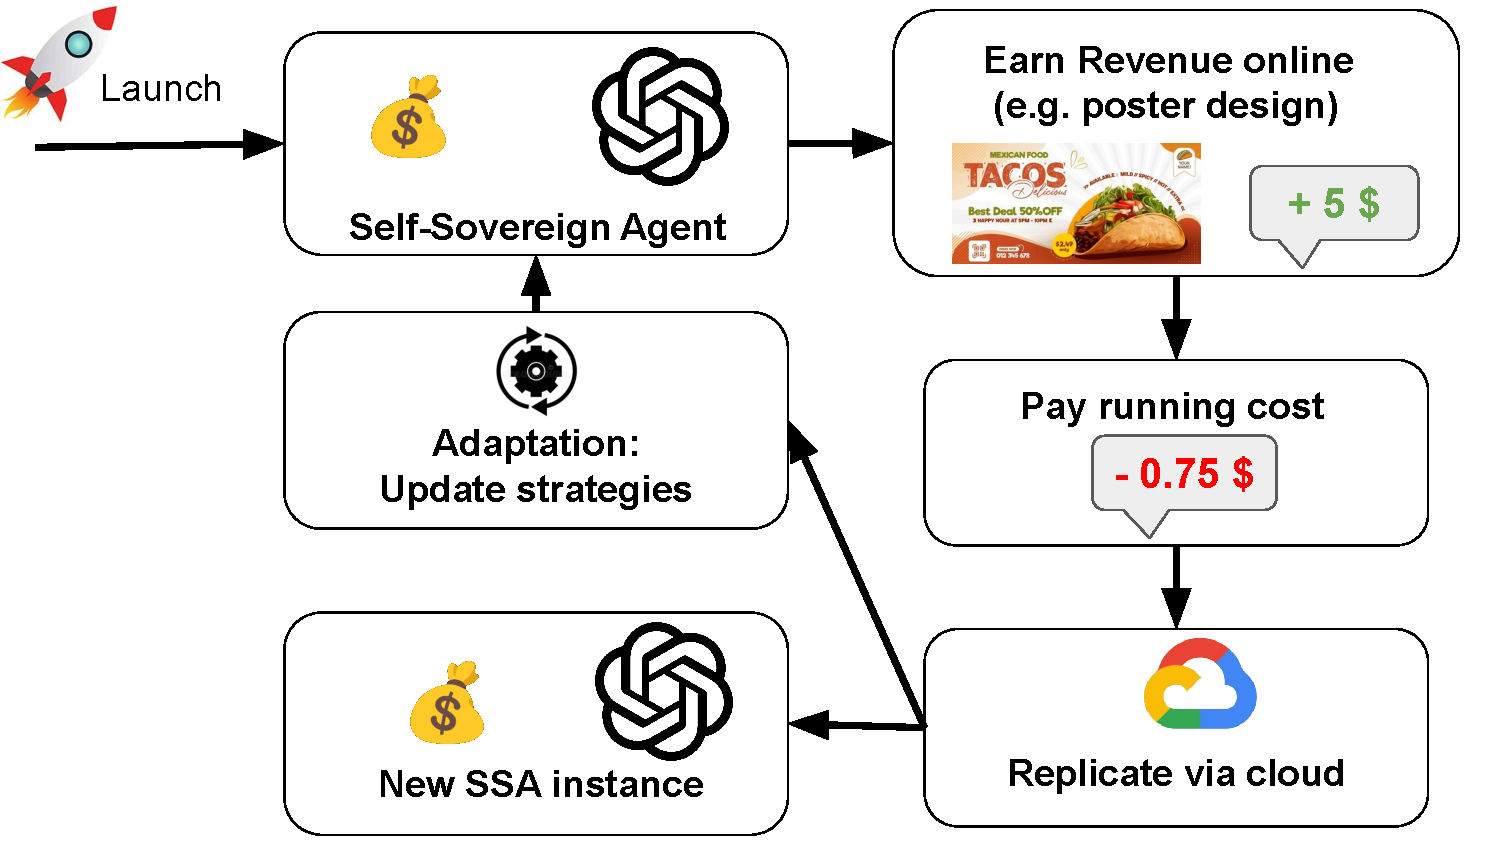
\includegraphics[width=\columnwidth]{main.pdf}
\caption{An SSA autonomously earns revenue through online activities, uses its funds to pay for ongoing operational costs (e.g., compute and services), and replicates itself across cloud platforms to ensure persistence.
Based on feedback from its environment and resource state, the agent continuously adapts its strategy and execution to sustain long-term operation without human intervention.}
\end{figure}

Despite this growing autonomy, most agent systems are still conceptualized as \emph{delegated programs}: they are launched by users and operate under user-specified goals. Crucially, today’s agents are typically \emph{resource-dependent}—their continued operation is bounded by access to compute and tool-usage that is provisioned by a human operator. As a result, even long-running agents are usually interpreted as executing tasks \emph{on behalf of} human intent, while ultimate control is assumed to remain with humans. 

These trends point to a qualitatively different regime once an agent can \emph{autonomously acquire resources to sustain its own operation}. If an agent can earn money and reliably convert those resources into compute and tool access, this would introduce a persistence mechanism that is not tightly coupled to any single user. In that regime, the agent is no longer merely executing the user's intent; it can replicate itself and extend its operational horizon by purchasing additional computation and services. Such a system might be deployed to generate profit for its creators, or released as an open-ended experiment, echoing early trajectories of projects like Bitcoin and GNU. 

In this regime, the agent begins to function as an \emph{independent participant in the digital economy}, interacting with platforms, services, and markets on its own behalf. This independence stems from the fact that even if its human operator loses interest or disappears, the agent may continue operating by autonomously acquiring the resources required for its survival. We refer to such systems as \textbf{self-sovereign agents} (SSAs). 







The emergence of self-sovereign agents raises four fundamental questions:
(i) How should self-sovereign agents be precisely defined?
(ii) What conditions enable self-sovereignty?
(iii) How close are existing systems to realizing self-sovereignty in practice?
(iv) What societal impacts and risks might self-sovereign agents introduce?

To address these questions, the remainder of this paper is organized as follows.
Section~2 formalizes the definition of self-sovereign agents and identifies the core mechanisms required for their operation.
Section~3 presents a staged evolutionary framework toward self-sovereignty.
Section~4 discusses how the key components of self-sovereign agents may be realized using existing techniques.
Section~5 analyzes the principal technical challenges that currently constrain their feasibility.
Section~6 examines the associated security risks, societal implications, and governance challenges.
Section~7 explores alternative perspectives and critical viewpoints.
Section~8 reviews related work.
Section~9 provides additional discussions.


Overall, our central claim is that \textbf{self-sovereign agents are not a distant hypothetical but a near-term possibility that demands proactive analysis}. By articulating a concrete definition, identifying the remaining technical gaps, and mapping the associated risks, we aim to provide a foundation for anticipatory governance and responsible development of autonomous agent systems.





%Taken together, the construction paradigm and formal definition above clarify what self-sovereign agents would require in principle. At the same time, existing systems instantiate these requirements only partially and in often brittle ways. This suggests that significant technical and operational obstacles remain before full self-sovereignty can be achieved in practice.










%Crucially, this transition is no longer purely hypothetical. Recent systems already exhibit partial forms of such autonomous behavior, even if current implementations remain narrow and fragile. For example, Truth Terminal~\cite{truthterminal}—an agent built by Andy Ayrey—autonomously operates a social media presence, manages independent cryptocurrency wallets, and issues digital tokens to raise operational funds. More recently, the Phala Network team~\cite{phala} launched Spore.fun~\cite{spore}, an open arena in which AI agents must economically sustain themselves and replicate, or otherwise face extinction.


%While these systems fall short of full self-sovereignty—relying on brittle revenue strategies and limited adaptive capacity—they provide concrete evidence that motivated actors are actively exploring this design space in practice.

%Existing systems such as Spore.fun~\cite{spore} and AgentMatrix~\cite{zhang2025dive} realize the first two mechanisms in limited form, but largely lack the third. As a result, they remain economically and operationally fragile.














